\documentclass{standalone}
\usepackage{tikz}
\usetikzlibrary{positioning, shapes.misc}

\begin{document}

\begin{tikzpicture}[
    box/.style={draw, minimum width=1.5cm, minimum height=0.8cm, rounded corners=0.2cm},
    arrow/.style={->, >=stealth},
    node distance=0.5cm and 0.2cm
]

% Placeholder image
\node[inner sep=0, outer sep=0] (image) at (0,0) {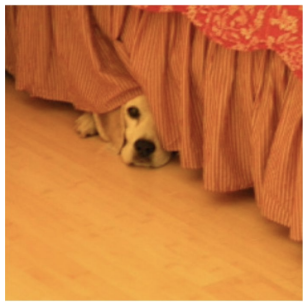
\includegraphics[width=5cm,height=5cm]{tikz/chapter7 - Sampling.png}};

\node[box, right=0.4cm of image, yshift=1cm, fill=gray!10] (the) {The};
\node[box, below=0.2cm of the, fill=gray!10] (a) {A};
\node[box, below=0.2cm of a, fill=gray!10] (one) {One};
\node[above=0.2cm of the] (p1) {$p_1$};

\node[box, right=1cm of the, fill=gray!10] (dog) {dog};
\node[box, below=0.2cm of dog, fill=gray!10] (yellow) {yellow};
\node[box, below=0.2cm of yellow, fill=gray!10] (cat) {cat};
\node[above=0.2cm of dog] (p2) {$p_2$};

\node[box, right=1cm of dog, fill=gray!10] (is) {is};
\node[box, below=0.2cm of is, fill=gray!10] (dog2) {dog};
\node[box, below=0.2cm of dog2, fill=gray!10] (sitting) {sitting};
\node[above=0.2cm of is] (p3) {$p_3$};

\node[box, right=1cm of is, fill=gray!10] (hiding) {hiding};
\node[box, below=0.2cm of hiding, fill=gray!10] (is2) {is};
\node[box, below=0.2cm of is2, fill=gray!10] (on) {on};
\node[above=0.2cm of hiding] (p4) {$p_4$};

\node[box, right=1cm of hiding, fill=gray!10] (stop) {STOP};
\node[box, below=0.2cm of stop, fill=gray!10] (sitting2) {sitting};
\node[box, below=0.2cm of sitting2, fill=gray!10] (the2) {the};
\node[above=0.2cm of stop] (p5) {$p_5$};

\draw[arrow, thick] (the) -- (dog);
\draw[arrow, thick] (a.east) -- (cat.west);
\draw[arrow, thick] (one.east) -- (yellow.west);
\draw[arrow, thick] (dog) -- (is);
\draw[arrow, thick] (dog.east) -- (sitting.west);
\draw[arrow, thick] (yellow) -- (dog2);
\draw[arrow, thick] (is) -- (hiding);
\draw[arrow, thick] (dog2) -- (is2);
\draw[arrow, thick] (is.east) -- (on.west);
\draw[arrow, thick] (hiding) -- (stop);
\draw[arrow, thick] (is2) -- (sitting2);
\draw[arrow, thick] (on) -- (the2);

\end{tikzpicture}

\end{document}